\documentclass[9pt]{beamer}
%
% Choose how your presentation looks.
%
% For more themes, color themes and font themes, see:
% http://deic.uab.es/~iblanes/beamer_gallery/index_by_theme.html
%
\mode<presentation>
{
  \usetheme{Singapore}     % or try Darmstadt, Madrid, Warsaw, ...
  \usecolortheme{default} % or try albatross, beaver, crane, ...
  \usefonttheme{default}  % or try serif, structurebold, ...
  \setbeamertemplate{navigation symbols}{}
  \setbeamertemplate{caption}[numbered]
} 

\AtBeginSection[]{
  \begin{frame}
  \vfill
  \centering
  \begin{beamercolorbox}[sep=8pt,center,shadow=true,rounded=true]{title}
    \usebeamerfont{title}\insertsectionhead\par%
  \end{beamercolorbox}
  \vfill
  \end{frame}
}

%\usepackage{ctex}
\usepackage[english]{babel}
\usepackage[utf8x]{inputenc}
\usepackage{graphicx}
%\usepackage{caption}
\usepackage{tikz}
\usepackage[normalem]{ulem}
\usepackage{hyperref}

%%%%%%%%%% Start TeXmacs macros
\newcommand{\Epsilon}{\mathrm{E}}
\newcommand{\mathd}{\mathrm{d}}
\newcommand{\tmop}[1]{\ensuremath{\operatorname{#1}}}
%%%%%%%%%% End TeXmacs macros

\title[]{Introduction to Generative Adversarial Network}
\author{Qiang Luo\\ hzluoqiang@corp.netease.com \\ luoq08@gmail.com}
%\institute{Where You're From}
\date{\today}

%\graphicspath{{GAN_figures}}

\begin{document}

\begin{frame}
  \titlepage
\end{frame}

% Uncomment these lines for an automatically generated outline.
\begin{frame}{Outline}
 \tableofcontents
\end{frame}

\section{Introduction}

\begin{frame}{Generative Model}

  \begin{itemize}
  \item Supervised Learning: discriminative vs generative model

    $P(y|x)$ or $f(x)$ vs $P(x,y)$
  \item Unsupervised Learning: learn the true data distribution $P_r(x)$
    \begin{itemize}
    \item explicitly learn the distribution
      \begin{figure}[!]
	\centering
	% http://scikit-learn.org/stable/auto_examples/mixture/plot_gmm_pdf.html
        \includegraphics[height=0.25\textheight]{GAN_figures/sphx_glr_plot_gmm_pdf_0011.png}
      \end{figure}
    \item hard to define for natural data
    \item generate sample directly
      \begin{center}
        \includegraphics[height=0.25\textheight]{GAN_figures/sample_generation.png}
      \end{center}
    \end{itemize}
  \end{itemize}
\end{frame}

\begin{frame}{Taxonomy of Generative Models}
  \includegraphics[height=0.8\textheight]{GAN_figures/taxonomy.png}
\end{frame}

\section{Application}
\begin{frame}{Super Resolution}
  \emph{Ledig et al 2016}
  \includegraphics[width=0.8\textwidth]{GAN_figures/SR.png}
\end{frame}

\begin{frame}{Image to Image Translation}
  \emph{Isola et al 2016}
  \includegraphics[width=0.8\textwidth]{GAN_figures/image_to_image_translation.png}
\end{frame}

\begin{frame}{Text to Image Synthesis}
  \emph{Generative Adversarial Text-to-Image Synthesis, Reed et al 2016}
  \includegraphics[width=0.8\textwidth]{GAN_figures/text_to_image_coco_samples.jpg}
\end{frame}

\begin{frame}{Image Generation}
  Use DCGAN
  \url{https://www.facebook.com/soumith/posts/10154442598946002}
  \includegraphics[height=0.8\textheight]{GAN_figures/DCGAN_manga.jpg}
\end{frame}

\begin{frame}{Image Generation}
  \includegraphics[height=0.8\textheight]{GAN_figures/DCGAN_album.jpg}
\end{frame}

\begin{frame}{Image Generation}
  \includegraphics[width=0.8\textwidth]{GAN_figures/DCGAN_chinese_character.jpg}
\end{frame}

\section{GAN}
\begin{frame}{GAN}
  \begin{itemize} 
  \item \emph{Generative adversarial nets (2014), I. Goodfellow et al.}
  \item min-max game for $D$ and $G$
  %generator $G$ generate sample, discriminater $D$ try to predict whether sample is generated or not
    \begin{center}
      %	\footnote{\tiny{\url{https://medium.com/@devnag/generative-adversarial-networks-gans-in-50-lines-of-code-pytorch-e81b79659e3f}}}
      \includegraphics[height=0.3\textheight]{GAN_figures/gan_concept.png}
      % https://www.slideshare.net/ckmarkohchang/generative-adversarial-networks?qid=e7715577-fcdb-4791-b42e-8e8e75465689&v=&b=&from_search=2
      \includegraphics[height=0.3\textheight]{GAN_figures/V(D,G).png}
    \end{center}
  $$ \min_G \max_D V(D,G) = E_{x \sim P_r (x)} \log (D (x)) + E_{z \in P_z
    (z)} \log (1 - D (G (z))) $$
  \item Find the Nash Equilibrium
  \item Fixed $G$, $D$ solve classification with log loss
  \item Fixed $D$, $G$ minimize $\log(1-D(G(z)))$
  \end{itemize}
\end{frame}

\begin{frame}{Algorithm}
    \includegraphics[height=0.5\textheight]{GAN_figures/gan_algo.png}

    \includegraphics[width=0.6\textwidth]{GAN_figures/gan_algo_step.png}
\end{frame}

\begin{frame}{Global minimum}
%  \begin{textblock*}{0.3\textwidth}(0.7\textwidth,0.2\textheight) % {block width} (coords)
  %\end{textblock*}
  \begin{itemize}
  \item Fixed $G$, optimal $D$ is $$ D^*(x)=\frac{P_r(x)}{P_r(x)+P_g(x)}$$
  \item With above solution, $G$ minimize $E_{x \sim P_r (x)} \log
    \frac{P_r (x)}{P_r (x) + P_g (x)} + E_{x \sim P_g (x)} \log
    \frac{P_g (x)}{P_r (x) + P_g (x)}=$
    $$2 \text{KS} (P_r, P_g) - \log (4) $$
  \item global minimum when $P_g=P_r$ with value of $-\log(4)$
  \item convergence in practice?
  \end{itemize}
\end{frame}

\begin{frame}{Problem of training}
  \begin{itemize}
  \item
      In practice, we modify G (sample generation function) and D
      (density ratio), not densities
  \item
      We represent G and D as highly non-convex parametric functions
  \item
    “Oscillation”: can train for a very long time, generating very many
    different categories of samples, without clearly generating better samples
  \item \emph{Mode collapse}: generated data is not diverse
  \end{itemize}
  \includegraphics[height=0.3\textheight]{GAN_figures/mode_collapse.png}
\end{frame}
\begin{frame}{Some tricks}
  \begin{itemize}
  \item minimize $-\log(D(G(z)))$ instead of $\log(1-D(G(z)))$ to
    prevent saturation when $G$ is poor and $D$ is confident
  \item
    $D$ must be synchronized well with G during training
  \item
    in particular, G must not be trained too much without updating D
    to prevent mode collapse
  \end{itemize}
\end{frame}

\begin{frame}{Result}
  \includegraphics[height=0.8\textheight]{GAN_figures/gan_result.png}
\end{frame}

\section{DCGAN}

\begin{frame}{Contribution}
  \begin{itemize}
  \item \emph{Unsupervised representation learning with deep convolutional generative adversarial networks (2015), A. Radford et al.}
  \item GAN for image generation
  \item identified a family of architectures that resulted in stable
    training across a range of datasets
  \item use feature from $D$ for classification
  \item arithmetic operation of latent vector
  \end{itemize}
\end{frame}

\begin{frame}{Architecture Guideline}
  \small{
  \begin{itemize}
  \item Replace any pooling layers with strided convolutions – this
    allows the network to learn its own spatial downsampling.
  \item 
    Remove any fully connected hidden layers on top of convolutional
    features. The authors found that connecting the highest convolutional
    features to the input and output respectively of the generator and
    discriminator worked well.
  \item 
    Use batch normalization, which stabilizes learning by normalizing the
    input to each unit to have zero mean and unit variance.
  \item 
    Use ReLU activation for all generator layers, except for the final
    output layer where tanh works better Use Leaky ReLU activation for all
    discriminator layers. (We can update that advice to PReLUs now)
  \end{itemize}}
\end{frame}

\begin{frame}{Architecture}
  \includegraphics[height=0.5\textheight]{GAN_figures/DCGAN_G.png}
  \begin{itemize}
  \item some hyper parameter tuning
  \item trained on three datasets, Large-scale Scene Understanding (LSUN) (Yu et al., 2015),
Imagenet-1k and a newly assembled Faces datase
  \end{itemize}
\end{frame}

\begin{frame}{Convolution and Transposed Convolution}
  \begin{itemize}
  \item \url{https://github.com/vdumoulin/conv_arithmetic}
  \item Convolution with kernel $3\times 3$, no padding, stride 1 for $4\times 4$ input produce $2\times 2$ output
  \item represent the transformation in matrix $4\times 9$ matrix $C$
  \includegraphics[width=0.8\textwidth]{GAN_figures/conv_C.png}
  \item in forward pass $y=C x$, in backward pass $dx = C^T dx$
  \item the transform defined by $C^T$ is called \emph{transposed convolution}, or \emph{fractionally strided convolution}, \sout{\emph{deconvolution}}
  \item It's another convolution with kernel $3\times 3$, pad 2, stride 1
  \end{itemize}

  \begin{center}
    \includegraphics[width=0.25\textwidth]{GAN_figures/no_padding_no_strides-0.png}
    \includegraphics[width=0.25\textwidth]{GAN_figures/no_padding_no_strides_transposed-0.png}
  \end{center}
\end{frame}

\begin{frame}{Generated Sample}
  \includegraphics[height=0.8\textheight]{GAN_figures/DCGAN_rooms.png}
\end{frame}

\begin{frame}{Usage in classification}
  \begin{quote} To evaluate the quality of the representations
    learned by DCGANs for supervised tasks, we train on Imagenet-1k
    and then use the discriminator’s convolutional features from all
    layers, maxpooling each layers representation to produce a 4 × 4
    spatial grid. These features are then flattened and concatenated
    to form a 28672 dimensional vector and a regularized linear L2-SVM
    classifier is trained on top of them.
  \end{quote}
  \begin{center}
    \includegraphics[width=0.8\textwidth]{GAN_figures/DCGAN_CIFAR_classification.png}
  \end{center}
\end{frame}

\begin{frame}{ Vector Arithmetic on face samples}
  \includegraphics[height=0.8\textheight]{GAN_figures/DCGAN_z_arithmetic.png}
  \includegraphics[width=0.5\textwidth]{GAN_figures/DCGAN_z_arithmetic_pose.png}
\end{frame}

\section{W-GAN}

\begin{frame}{Contribution}
  \begin{itemize}
    \item \emph{Towards principled methods for training generative adversarial networks(2017), M. Arjovsky et al}
    \item \emph{Wasserstein GAN (2017), M. Arjovsky et al}
    \item find the reason why GAN training is hard
    \item algorithm with good theory and works
    \item no more mode collapse?
    \item no more architecture design
    \item sensible loss metric for training
  \end{itemize}
  \includegraphics[width=0.8\textwidth]{GAN_figures/WGAN_reddit.png}
\end{frame}

\begin{frame}{Why is GAN hardy to train?}
  \begin{itemize}
  \item MLE maximize $\frac{1}{m} \sum_{i = 1}^m \log (P_g (x_i))$, which is minimize $\text{KL}(P_r||P_g)$
  \[ \text{KL} (P_r, P_g) = \int P_r (x) \log \frac{P_r (x)}{P_g (x)} \mathd x
\]
  \item GAN minimize $\text{JS}(P_r, P_g)$(original, minimize $\log(1-D(G(x)))$ for $G$)
  \item if $P_r(x)\gg P_g(x)$(mode dropping) KL goes to inf; if $P_r(x)\ll P_g(x)$(generate bad sample) KL goes to zero
  \item \emph{Manifold hypothesis}: Natural data forms lower
    dimensional structures (manifolds) in the embedding space
  \item natural image embeded in space of all possible image $R^{3\times 64\times64}$; $g_\theta$ map $R^{100}$ to $R^{3\times 64\times64}$
  \item support for $P_r$ and $P_g$ almost never intersect;
    $\text{JS}(P_r,P_g)=\log{2}$, $\text{KL}(P_r, P_g)=\infty$,
    $\text{KL}(P_g, P_r)=\infty$
  \item If $D$ goes to optimal, the loss for $G$ is $KS$ and
    gradient from $D$ will go to zero
  \end{itemize}
\end{frame}

\begin{frame}{Evidence from DCGAN training}
  \begin{itemize}
  \item when $D$ is near optimal, we can not train $G$
  \item when $D$ is far from optimal, it's bad
  \item the coordinance is hard
  \end{itemize}
  \includegraphics[height=0.4\textheight]{GAN_figures/GAN_loss_of_D.png}
  \includegraphics[height=0.4\textheight]{GAN_figures/GAN_gradient_of_G.png}
\end{frame}

\begin{frame}{Why is GAN hard to train?}
  \begin{itemize}
  \item usually $-\log(D(G(x)))$ is optimized for $G$
  \item in this case the loss is $$\text{KL}(P_g||P_r)-2 \text{JS}(P_g||P_r)$$
  \item this loss(when stably trained) penalize generating bad sample and tolerate mode loss
  \item in this case the gradients for $G$ is unstable
  \end{itemize}
  \includegraphics[height=0.4\textheight]{GAN_figures/GAN_gradient_of_G_2.png}
\end{frame}

\begin{frame}{Wasserstein metric}
  \begin{itemize}
  \item \emph{Wasserstein metric} (transportation metric, earth mover's distance)
    \[ W (P, Q) = \inf_{\gamma \in \Gamma} E_{x, y \sim \gamma} (\| x - y \|) =
   \inf_{\gamma \in \Gamma} \int_{X, Y} \| x - y \| \gamma (x, y) \mathd x
   \mathd y \]
    where $\Gamma$ is the joint distribution on $(x,y)$ with marginal
    distribution $P,Q$
  \item $\gamma(x,y)$ is the quantity we transport from $x$ to $y$,
    the marginal requirement makes sure $P$ is transported to $Q$
  \begin{block}{Uniform distributions on parallel lines}
    \begin{center}
    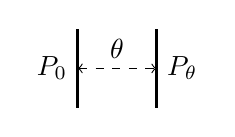
\begin{tikzpicture}
      \centering
      \draw[line width=1pt] (0,0) -- (0,1) node[pos=0.5, left]{$P_0$};
      \draw[line width=1pt] (1,0) -- (1,1) node[pos=0.5, right]{$P_\theta$};
      \draw[dashed, <->] (0, 0.5) -- (1, 0.5) node[pos=0.5, above]{$\theta$};
    \end{tikzpicture}
    \end{center}
  \end{block}
    \begin{itemize}
    \item $\text{KL}(P_0, P_\theta)=+\infty$ if $\theta \not= 0$ else $0$
    \item $\text{JS}(P_0, P_\theta)=\log(2)$ if $\theta \not= 0$ else $0$
    \item $W(P_0, P_\theta)=|\theta|$
    \end{itemize}
  \item For $P_r$ and $P_\theta$ generate from $g_\theta(z)$, $W(P_r,
    P_\theta)$ is good(continuous, differentiable, ...)
  \item sequence converges in KL, JS if it converges in $W$
  \end{itemize}
\end{frame}

\begin{frame}{Use Wasserstein metric}
  \begin{itemize}
  \item a result from \emph{Kantorovich-Rubinstein duality}
    \[ W (P, Q) = \frac{1}{K} \sup_{\| f \|_L \leqslant K} E_{x \in P} f (x) -
   E_{x \in Q} f (x) \] where $\|f\|_L\leqslant K$ means $\| f (x) - f
   (y) \| \leqslant K \| x - y \|, \forall x, y$ ($K$-Lipschitz functions)
 \item whose parameter $w$ clamped to $[-c, c$]
   \[ \min_{\theta} \max_w E_{x \sim P_r} (f_w (x)) - E_{z \sim P_z} (f_w
   (g_{\theta} (z))) \]
   The original GAN is
  $$ \min_G \max_D V(D,G) = E_{x \sim P_r} \log (D (x)) + E_{z \in P_z
   } \log (1 - D (G (z))) $$
 \end{itemize}
\end{frame}

\begin{frame}{Algorithm}
WGAN training becomes unstable at times when one uses a momentum based
optimizer such as Adam, use momentum free optimizer
\includegraphics[width=0.8\textwidth]{GAN_figures/WGAN_algo.png}
\end{frame}

\begin{frame}{On 1d Gaussian}
  \includegraphics[width=0.8\textwidth]{GAN_figures/WGAN_vs_GAN_gaussian.png}
\end{frame}

\begin{frame}{loss vs quality for WGAN}
  \includegraphics[height=0.8\textheight]{GAN_figures/loss_vs_quality_WGAN.png}
\end{frame}

\begin{frame}{loss vs quality for original GAN}
  \includegraphics[height=0.8\textheight]{GAN_figures/loss_vs_quality_GAN_original.png}
\end{frame}

\begin{frame}{loss vs quality for GAN}
  \includegraphics[height=0.8\textheight]{GAN_figures/loss_vs_quality_GAN.png}
\end{frame}

\begin{frame}{image samples for different network}
  DCGAN
  \includegraphics[height=0.2\textheight]{GAN_figures/samples_DCGAN.png}

  DCGAN without tricks
  \includegraphics[height=0.2\textheight]{GAN_figures/samples_DCGAN_no_trick.png}

  mlp
  \includegraphics[height=0.2\textheight]{GAN_figures/samples_mlp.png}
\end{frame}

\begin{frame}{Discuss}
  \begin{itemize}
  \item How to estimate $K$ from $c$ and architecture?
  \item How to compare between $c$ and architectures?
  \end{itemize}
\end{frame}

\section{Reference}

\begin{frame}{paper}
  \begin{itemize}
  \item \emph{Generative adversarial nets (2014), I. Goodfellow et al.}
  \item \emph{Unsupervised representation learning with deep
    convolutional generative adversarial networks (2015), A. Radford
    et al.}
  \item \emph{Towards principled methods for training generative
    adversarial networks(2017), M. Arjovsky et al}
  \item \emph{Wasserstein GAN (2017), M. Arjovsky et al}
  \end{itemize}
\end{frame}

\begin{frame}{web}
  \begin{itemize}
  \item
    \href{https://blog.acolyer.org/2017/03/02/unsupervised-learning-and-gans/}{Unsupervised
      learning and GANs}
  \item
    \href{http://www.alexirpan.com/2017/02/22/wasserstein-gan.html}{Read-through:
      Wasserstein GAN}
  \item \url{https://zhuanlan.zhihu.com/p/25071913}
  \item
    \url{https://www.reddit.com/r/MachineLearning/comments/5qxoaz/r_170107875_wasserstein_gan/}
  \item \href{https://arxiv.org/abs/1701.00160}{(NIPS 2016
    tutorial)Generative Adversarial Networks (GANs)},
    \href{http://www.iangoodfellow.com/slides/2016-12-04-NIPS.pdf
    }{slide}
  \item \url{https://github.com/vdumoulin/conv_arithmetic}
  \item
    \href{https://github.com/terryum/awesome-deep-learning-papers}{Awesome
      - Most Cited Deep Learning Papers}
  \item \url{https://www.facebook.com/soumith/posts/10154442598946002}
  \end{itemize}
\end{frame}


\end{document}
